\documentclass[12pt]{article}

% La gestion des fontes, sachant que ce document est sensé
% être compilé au moyen de XeLaTeX
%\usepackage{fontspec,xltxtra}

% Pour permettre la redéfinition des dimensions
\usepackage[a4paper]{geometry}

% Pour le support du français
\usepackage[francais]{babel}

% Les polices à utiliser
%\newcommand{\fontsphil}{
 % \defaultfontfeatures{Mapping=tex-text}
  %\defaultfontfeatures{Ligatures=TeX}
  %\setmainfont{Linux Libertine O}
  %\setsansfont{Liberation Sans}
  %\setmonofont[Scale=.9]{Ubuntu Mono}
  %\newfontfamily{\hwfont}{Comic Sans MS}
  %\newfontfamily{\fatfont}{Arial Black}
  %\newfontfamily{\authorfont}{Liberation Serif}
  %\newfontfamily{\spacefont}{Liberation Mono}
  %\fontspec[SmallCapsFont={Arial Black}]{Arial Black}
%}
%\fontsphil

% Des polices pour quelques caractères spéciaux
\usepackage{wasysym}
\usepackage{pifont}

% Gestion des images
\usepackage{graphicx}

% Gestion des couleurs
\usepackage{color}
\definecolor{fondsection}{rgb}{.9,.9,.9}

% Gestion des espaces
\usepackage{xspace}

% Gestion des URL et liens hypertexte
\usepackage{hyperref}

% Configuration des dimensions
\geometry{%
  left=20mm,width=165mm,
  top=15mm,height=267mm,
  footskip=15mm}

% Le titre
\title{Mon super rapport de stage}
\author{Alain Térieur}
\date{Année universitaire 2022--2023}

% Une macro
\newcommand{\oula}{(\textbf{???})}

% Macro pour page vide sans numérotation
\usepackage{afterpage}
\newcommand\myemptypage{
    \null
    \thispagestyle{empty}
    \addtocounter{page}{-1}
    \newpage
    }

% Packet pour les tableaux
\usepackage{array}
\usepackage{tabularx}

%======================================================================
% D É B U T   D U   D O C U M E N T
%======================================================================

\begin{document}

  \thispagestyle{empty}
  \begin{center}
    
\includegraphics[width=12cm]{images/Logo_IUT-UL_dept_info.png}
  \end{center}

  \vspace{1cm}

  \noindent
  {\large
    IUT Nancy Charlemagne\\
    Université de Lorraine\\
    2 ter boulevard Charlemagne\\
    BP 55227\\
    54052 Nancy Cedex\\[5mm]
    Département informatique
  }

  \vspace{5cm}

  \begin{center}
    {\huge
      \textbf{Synthèse des TD}
    }
  \end{center}

  \vspace{5cm}

  % \vspace{2cm}
  \vfill

  {\Large
    \noindent
    Etudiant : Théo Eisenbart\\
    Année universitaire 2022--2023
  }
  % Ajout d'une page vide
  \newpage
  \thispagestyle{empty}
  \mbox{}
  \newpage

  \newpage
  % Table des matières
  \tableofcontents

  \newpage

  \section{Efficacité de l'environnement de travail}

    \subsection{TD-1 : La souris}
    \vspace{0.3cm}

  \begin{itemize}
    \item \textbf{Désactiver votre souris au noveau système avec la commande xinput}
  \end{itemize}

  \vspace{0.3cm}
  \$ sudo xinput disable\{2,4,6\}
  \vspace{0.3cm}

  \begin{itemize}
    \item \textbf{Initialiser un fichier dans lequel nous allons lister tous les problèmes d'efficacité rencontrés pendant cette séance}
  \end{itemize}
  \vspace{0.3cm}

  \begin{tabular}{|c|p{5cm}|p{10cm}|}
    \hline
    \textbf{Priorité} & \textbf{Problème} & \textbf{Correctif}\\
    \hline
    1 & Logout difficile au clavier & Raccourci clavier \textbf{Ctrl+Alt+Suppr/Delete}\\
    \hline
    2 & Impossible d'éditer des documents PDF avec Google Drive & Utilisation de LaTeX\\
    \hline
    3 & Impossible d'avoir plusieurs terminaux en parallèle & Sous Terminator, \textbf{Ctrl+Shift+O} pour split le terminal verticalement,\newline \textbf{Ctrl+Shift+L} pour split le terminal horizontalement\\
    \hline
    4 & Naviguer dans discord sans la souris & \textbf{Tab} pour se déplacer de haut en bas, \textbf{Shift+Tab} pour aller de bas en haut \newline et \textbf{Ctrl+Tab} pour naviguer de gauche à droite\\
    \hline
    5 & Se déplacer dans un éditeur de text sans la souris & Utilisation de Vim\\
    \hline
    6 & Ouvrir les settings de notre environnement graphique & shortcut configurable dans les settings ex : \textbf{Alt+S}\\
    \hline
    7 & Accèder au navigateur de fichier & shotcut configurable dans les settings ex : \textbf{Alt+F}\\
    \hline
  \end{tabular}
\vspace{0.3cm}

	\subsection{TD-2 : Le clavier}
  \vspace{0.3cm}

  \begin{itemize}
	  \item \textbf{Identifier un site permettant de s'améliorer à taper au clavier}
  \end{itemize}

\vspace{0.3cm}
\href{https://10fastfingers.com/typing-test/french#}{Le site 10fastfingers} car :
 \vspace{0.3cm}
		\begin{itemize}
      \begin{itemize}
			  \item Il est gratuit
			  \item Il a de nombreuse langue à disposition
			  \item Il est très simple d'utilisation
      \end{itemize}
		\end{itemize}

\vspace{0.3cm}
\begin{itemize}
  \item \textbf{Screen de l'interface :}
\end{itemize}
\vspace{0.3cm}

\begin{center}
  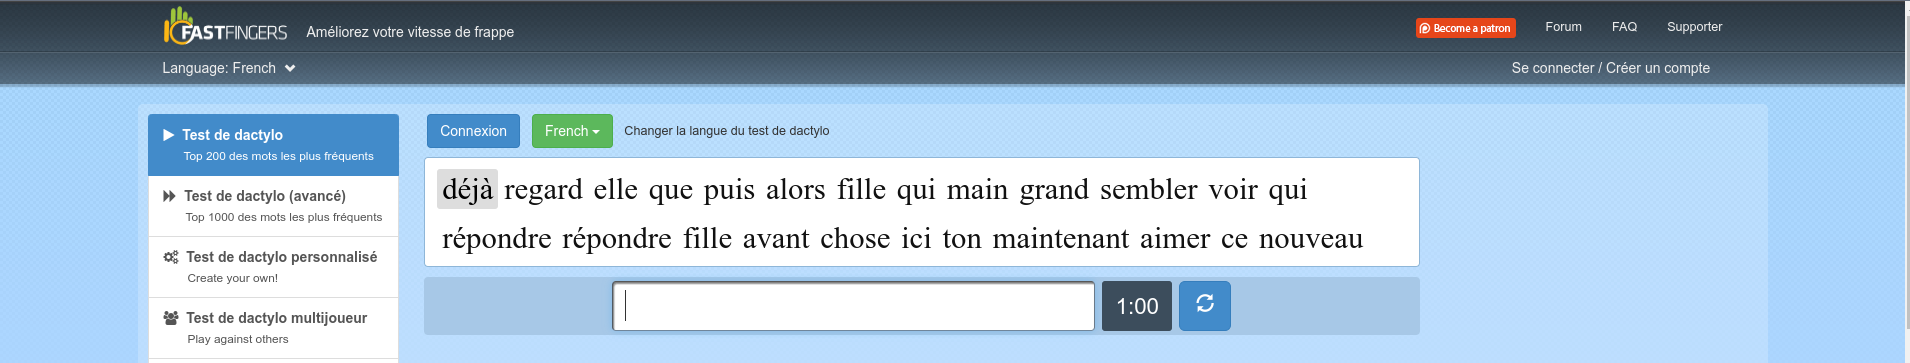
\includegraphics[width=12cm]{images/screen-10fastfingers.png}
\end{center}

\vspace{0.3cm}
\begin{itemize}
  \item \textbf{Quelque Résultat :}
\end{itemize}

\thispagestyle{empty}
\begin{center}
  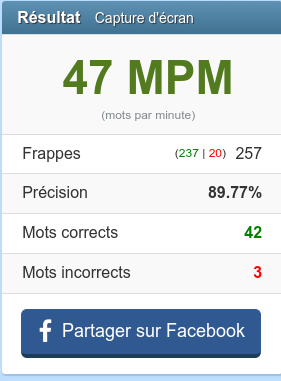
\includegraphics[width=4cm]{images/screen-resultat-1.png}\hfill
  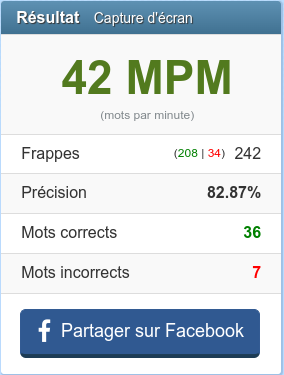
\includegraphics[width=4cm]{images/screen-resultat-2.png}\hfill
  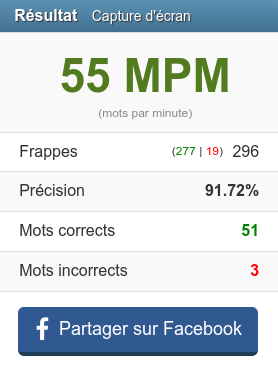
\includegraphics[width=4cm]{images/screen-resultat-3.png}
\end{center}
\vspace{0.3cm}

	\subsection{TD-3 : Le Shell}
  \vspace{0.3cm}

\begin{itemize}
  \item \textbf{Effectuer les tutoriels pour Vim et Emacs :}
\end{itemize}
\vspace{0.3cm}

J'ai choisie d'apprendre VIM car c'est le plus utilisé et il est plus pratique que Emacs

\vspace{0.3cm}

\begin{itemize}
  \item \textbf{Paramétrer GNU Readline :}
  \vspace{0.3cm}

  \$ set -o emacs \newline
  ou \newline
  \$ set -o vi \newline
\end{itemize}

\begin{itemize}
  \item \textbf{Tester les 2 modes, en choisir un :}
\end{itemize}
\vspace{0.3cm}

J'ai choisie le mode Emacs car c'est le mode que j'ai le plus utilisé donc celui avec lequel je me sens le plus à l'aise
c'est par ailleurs le mode par défaut ce qui me facilite grandement si je dois travailler sur une autre machine

\vspace{0.3cm}

\begin{itemize}
  \item \textbf{Paramétrer Emacs ou Vim comme étant éditeur par défaut en plus du mode de readline :}

  \vspace{0.3cm}

  Ligne à ajouter dans le .bashrc .zshrc :
  \vspace{0.3cm} \newline
  \$ export EDITOR="vim"
  \vspace{0.3cm} \newline
  Ligne à effectuer dans le terminal pour chnager de readline :
  \vspace{0.3cm} \newline
  \$ set -o emacs \newline
  \newline
  J'ai donc choisie comme configuration "vim" en éditeur de texte par défaut et Emacs comme readline
\end{itemize}

  \subsection{TD-4 : Bash history}
  \vspace{0.3cm}

\begin{itemize}
  \item \textbf{Regardez votre "history" :}

  \vspace{0.3cm}

  Voici ce qu'on obtient avec la commande : \$ history
\end{itemize}
\vspace{0.3cm}

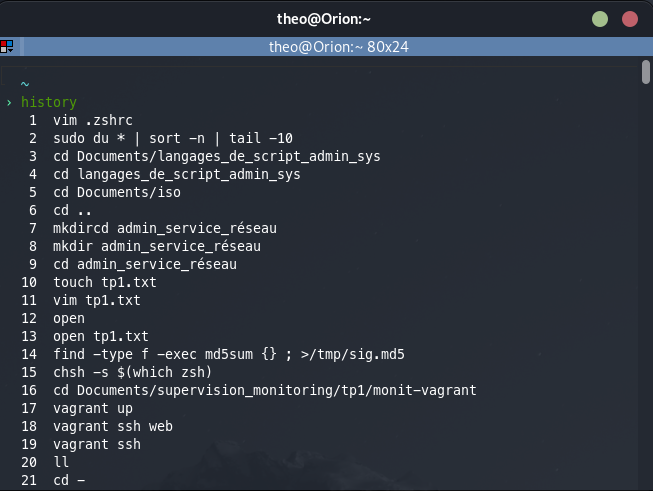
\includegraphics[width=11cm]{images/screen-term-td4.png}
\vspace{0.3cm}

\begin{itemize}
  \item \textbf{Y'a-t-il des informations sensibles ? Comment y rémédier ?}

  \vspace{0.3cm}

  Oui il y a des informations sensibles car cette commande montre toutes les commandes qui ont été tapé (dans mon cas dans zsh) \newline
  Mais il y a un moyen d'y remédier, autorisé la lecture au fichier ".zsh\_history" uniquement à root
\end{itemize}
\vspace{0.3cm}

\begin{itemize}
  \item \textbf{Un employé de longue date semble avoir un history très court, quelles sont les causes possibles ?}

  \vspace{0.3cm}

  L'employé semble avoir changé de shell en passant de bash à zsh, vue qu'on remarque qu'il a installé zsh
\end{itemize}
\vspace{0.3cm}

\begin{itemize}
  \item \textbf{Nos history sont souvent pollués par beaucoup de ls , cd , pwd ...
  Ces commandes sont tellement courtes que les taper entièrement est plus rapide.
  On veut éviter qu'elles n'apparaissent dans les résultats de recherche de
  l'history, comment faire ?}
  \vspace{0.3cm}

  Pour régler ce problème, il suffit d'ajouter un sed pour filtrer les commandes non désirées : \newline

  exemple : \$ history $|$ sed '/ls/d'

\end{itemize}

  \subsection{TD-5 : Bash aliases}
\vspace{0.3cm}

\begin{itemize}
  \item \textbf{Ecrire une bash function mkcd mondossier qui créé le dossier mondossier
  puis navigue dedans}
  \vspace{0.3cm}

  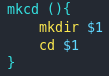
\includegraphics[width=3cm]{images/screen-mkcd-td5.png}
  \vspace{0.3cm}

  Dans cette bash function, on va prendre l'argument 1 qui est le chemin de création du dossier pour pouvoir
  l'inclure dans les 2 commandes en dessous.

\end{itemize}

\vspace{0.3cm}

\begin{itemize}
  \item \textbf{Ecrire une bash function gitemergency qui add, commit, et push tout son
  travail sur l'origin, permettant de ne rien perdre en cas d'alerte incendie}
  \vspace{0.3cm}

  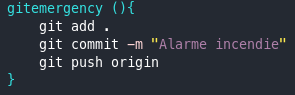
\includegraphics[width=7cm]{images/screen-gitemergency-td5.png}
  \vspace{0.3cm}

  Dans cette bash function, pas besoin de rentrer d'argument en plus, les commandes vont s'enchainer automatiquement
\end{itemize}

  \subsection{TD-8 : Custom-shortcut}
\vspace{0.3cm}

\begin{itemize}
  \item \textbf{Dans zsh, créer un raccourci Ctrl + Shift + A :}
  \vspace{0.3cm}

  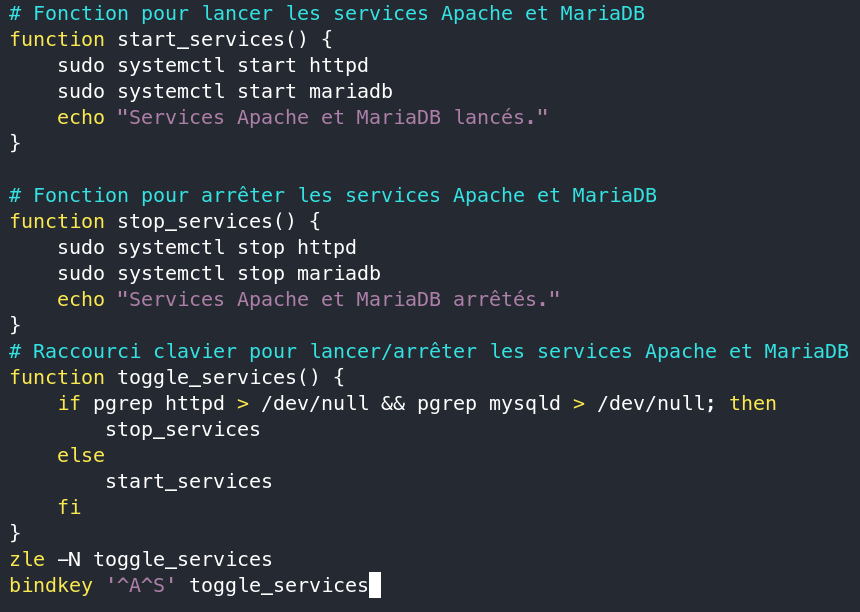
\includegraphics[width=10cm]{images/screen-td8.png}
  \vspace{0.3cm}

  Dans ce script j'ai intégré 3 fontions, 2 pour lancer et arrêter les services et la dernière pour le raccourci clavier.
\end{itemize}

  \subsection{TD-9 : Les terminaux}
\vspace{0.3cm}

\begin{itemize}
  \item \textbf{Installez et essayer 3+ émulateurs de terminaux parmi la liste précédente}
  \vspace{0.3cm}

  J'ai choisie de tester : Terminator, Gnome-terminal, et Putty
\end{itemize}
\vspace{0.3cm}

\begin{itemize}
  \item \textbf{Choisir un terminal et justifier pourquoi}
  \vspace{0.3cm}

  J'ai choisie d'utiliser Terminator, car il utilise le multiplexage, il dispose d'un grand nombre de raccourci pour passer
  d'un sous terminal à un autre, il dispose aussi d'une bonne documentation du à sa forte communauté
\end{itemize}

  \section{Client SSH}

    \subsection{TD-1 : Prise en main avec SSH}
    \vspace{0.3cm}

\begin{itemize}
  \item \textbf{Se connecter à la machine srv avec les utilisateurs alice, bob et carole sans utiliser vagrant ssh}
  \vspace{0.3cm}

  La commande pour se connecter en SSH est : \newline

  \$ ssh bob@10.0.0.1

\end{itemize}
\vspace{0.3cm}

\begin{itemize}
  \item \textbf{Vérifier qu'on est bien sur la machine Vagrant et pas en local}
  \vspace{0.3cm}

  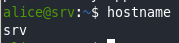
\includegraphics[width=4cm]{images/screen-ssh-td1.png}
  \vspace{0.3cm}

  On remarque que c'est le nom de la machine vagrant, donc je suis bien connecté dessus

\end{itemize}
\vspace{0.3cm}

\begin{itemize}
  \item \textbf{Consulter l' history local, que remarque-t-on ?}
  \vspace{0.3cm}

  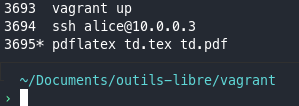
\includegraphics[width=4cm]{images/screen-ssh-td1-2.png}
  \vspace{0.3cm}

  On remarque que le mot de passe n'apparait pas dans le .bash\_history
\end{itemize}
\vspace{0.3cm}

  \subsection{TD 2 : Autenthification automatique}
  \vspace{0.3cm}

\begin{itemize}
  \item \textbf{Créer une paire de clés privée et publique à l'aide de ssh-keygen}
  \vspace{0.3cm}

  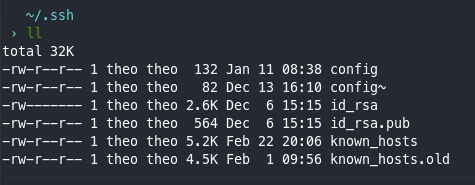
\includegraphics[width=7cm]{images/screen-ssh-td2.png}
  \vspace{0.3cm}

  Ma clé publique \(id\_rsa.pub\) et ma clé privée \(id\_rsa\) sont bien présente
\end{itemize}
\vspace{0.3cm}

\begin{itemize}
  \item \textbf{Utiliser la commande ssh-copy-id pour déposer la clé publique sur le compte alice@cli.
  Vérifier qu'on peut maintenant se connecter sans mot de passe}
  \vspace{0.3cm}

  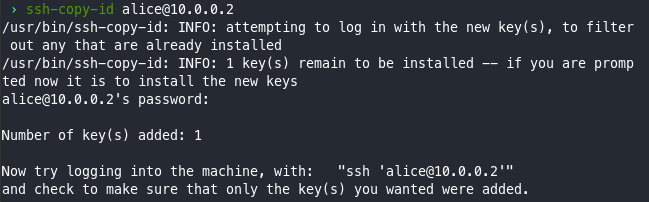
\includegraphics[width=10cm]{images/screen-ssh-td2-2.png}
  \vspace{0.3cm}

  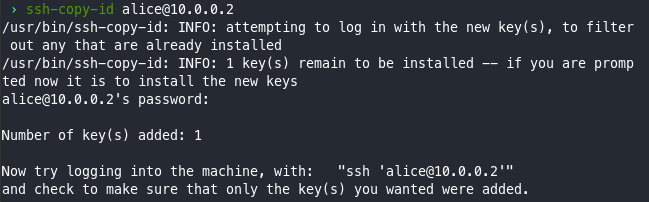
\includegraphics[width=9cm]{images/screen-ssh-td2-2.png}
  \vspace{0.3cm}

  La clé à bien été généré et déposé sur le compte alice@cli, on peut maintenant se connecter sans taper le mot de passe
\end{itemize}
\vspace{0.3cm}

\begin{itemize}
  \item \textbf{Déposer manuellement la clé publique sur le compte bob@cli}
  \vspace{0.3cm}

  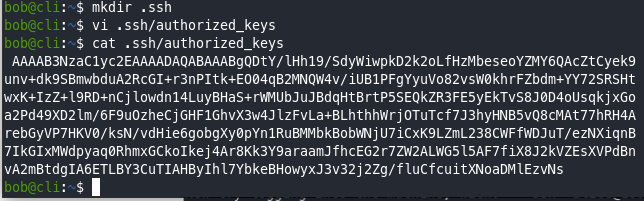
\includegraphics[width=9cm]{images/screen-ssh-td2-4.png}
  \vspace{0.3cm}

  Dans bob@cli j'ai créé le dossier .ssh ainsi que le fichier authorized\_keys auquel j'ai ajouté ma clé publique,
  et maintenant je peut me connecter sans avoir à taper le mot de passe avec cette commande : \newline

  
\includegraphics[width=8cm]{images/screen-ssh-td2-5.png}
  \vspace{0.3cm}

\end{itemize}
\vspace{0.3cm}

  \subsection{TD 3 : Known Hosts}
  \vspace{0.3cm}

\begin{itemize}
  \item \textbf{A l'aide de ssh-keygen et ssh-keyscan , ajouter la clé publique du serveur srv manuellement,
  décrire les étapes}
  \vspace{0.3cm}

  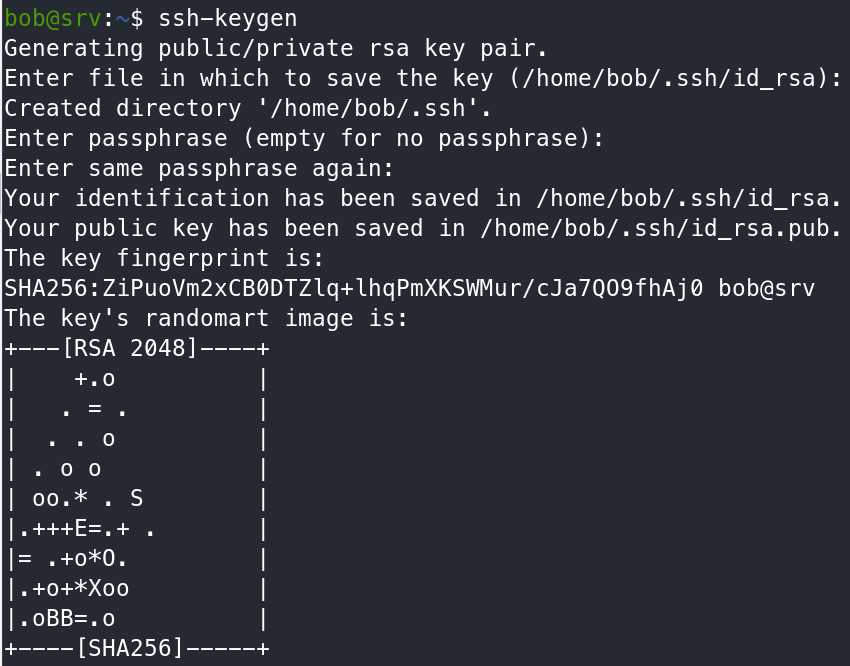
\includegraphics[width=8cm]{images/screen-ssh-td3-1.png}
  \vspace{0.3cm}

  j'ai créé la clé publique pour le serveur
  \vspace{0.3cm}

  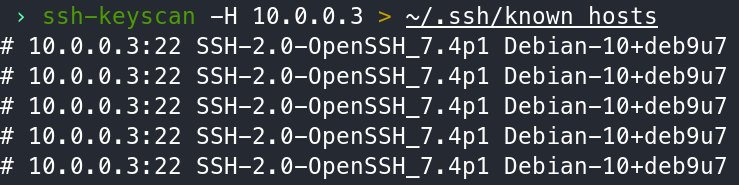
\includegraphics[width=8cm]{images/screen-ssh-td3-2.png}
  \vspace{0.3cm}

  Puis avec ssh-keyscan on récupère la clé publique pour la mettre dans notre Known-Hosts

\end{itemize}
\vspace{0.3cm}

\begin{itemize}
  \item \textbf{Créer un fichier de configuration pour SSH, vous permettant de vous connectersur le compte bob@cli
  en tapant ssh bc}
  \vspace{0.3cm}

  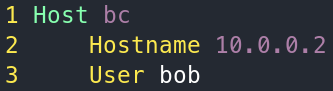
\includegraphics[width=4.5cm]{images/screen-ssh-td3-3.png}
  \vspace{0.3cm}

\end{itemize}
\vspace{0.3cm}

\begin{itemize}
  \item \textbf{Vérifiez que vous arrivez à vous connecter au compte alice@cli en utilisant SFTP.
  Copiez-y un fichier par SFTP, puis récupérez un autre fichier}
  \vspace{0.3cm}

  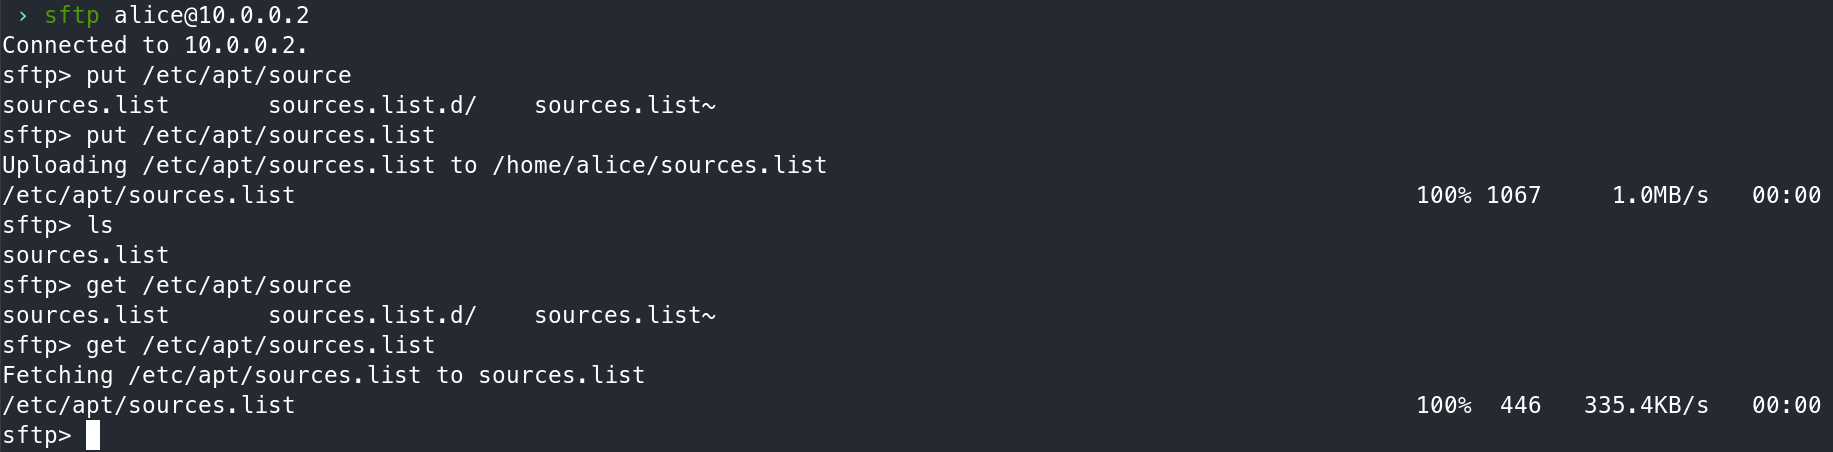
\includegraphics[width=15cm]{images/screen-ssh-td3-4.png}
\end{itemize}
\vspace{0.6cm}

\begin{itemize}
  \item \textbf{Vérifiez que vous arrivez à vous connecter au compte alice@cli avec SSHFS. Éditez un fichier distant
  avec un éditeur graphique (par exemple GVIM)}
  \vspace{0.3cm}

  
\includegraphics[width=9cm]{images/screen-ssh-td3-5.png}
  \vspace{0.3cm}

  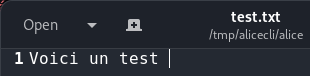
\includegraphics[width=8cm]{images/screen-ssh-td3-6.png}
  \vspace{0.3cm}

  J'arrive bien à monter dans /tmp/alicecli les "home" de tout les utilisateurs et j'arrive aussi à modifier des fichiers
  commme montré ci-dessus

\end{itemize}
\vspace{0.3cm}

\begin{itemize}
  \item \textbf{Vérifiez que la modification est bien répercutée sur la machine virtuelle alice@cli}
  \vspace{0.3cm}

  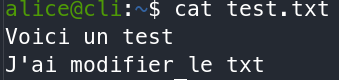
\includegraphics[width=7cm]{images/screen-ssh-td3-7.png}

\end{itemize}
\vspace{0.3cm}

  \subsection{TD-4 : Tunnel SSH}
  \vspace{0.3cm}

\begin{itemize}
  \item \textbf{Créer un tunnel SSH entre votre poste et srv à travers la machine cli}
  \vspace{0.3cm}

  La ligne de commande à éffectuer sur le poste est :
  \vspace{0.3cm}

  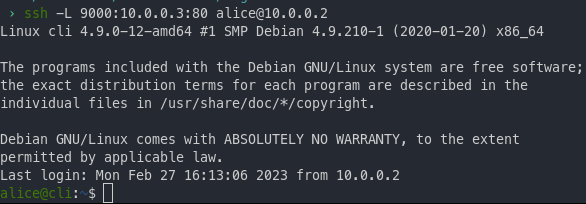
\includegraphics[width=9cm]{images/screen-ssh-td4-2.png}
  \vspace{0.3cm}

  Avec cette commande, la machine cli fait l'intermédiaire entre mon poste et srv, pour accèder au service de srv ma requête
  doit d'abord passer par la machine cli sur le port 9000 puis la machine cli envoie une requête à srv sur le port 80
\end{itemize}
\vspace{0.3cm}

\begin{itemize}
  \item \textbf{Tester en ouvrant un navigateur sur votre poste local à l'adresse
  http://localhost:8000/cgi-bin/test1.cgi}
  \vspace{0.3cm}

  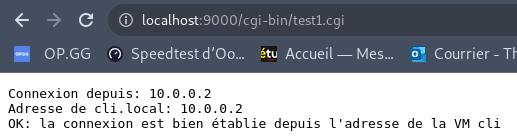
\includegraphics[width=9cm]{images/screen-ssh-td4-1.png}
  \vspace{0.3cm}

  J'arrive bien à accèder au service de srv par l'intermédiaire de la machine cli
\end{itemize}
\vspace{0.3cm}

  \subsection{TD-5 : SOCKS proxy}
  \vspace{0.3cm}

\begin{itemize}
  \item \textbf{Se connecter en SSH sur srv}
  \vspace{0.3cm}

  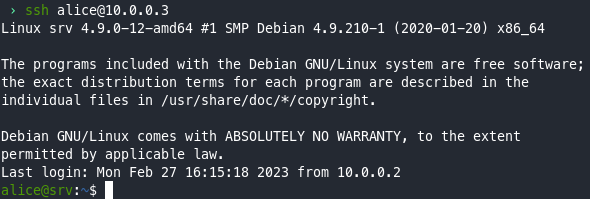
\includegraphics[width=9cm]{images/screen-ssh-td5-1.png}
  \vspace{0.3cm}

  je suis connecté au srv sur le compte alice
\end{itemize}
\vspace{0.3cm}

\begin{itemize}
  \item \textbf{Se connecter à cli en permettant à cli d’accéder à srv via un tunnel accessible par le port 9000}
  \vspace{0.3cm}

  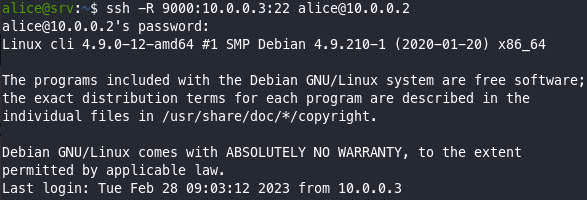
\includegraphics[width=9cm]{images/screen-ssh-td5-2.png}
  \vspace{0.3cm}

  maintenant le tunnel est bien créé
  \vspace{0.3cm}

  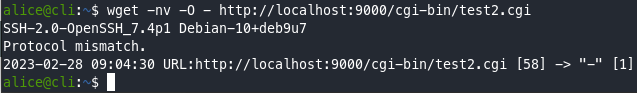
\includegraphics[width=9cm]{images/screen-ssh-td5-3.png}
  \vspace{0.3cm}

  La machine cli n'arrive pas à accèder au service de srv, hônnétement, j'ai pas trop compris cette partie du td
\end{itemize}
\vspace{0.3cm}

  \subsection{TD-6 : X11 Forwarding}
  \vspace{0.3cm}

\begin{itemize}
  \item \textbf{Installer une application graphique sur cli, ainsi que xauth}
  \vspace{0.3cm}

  \$ apt install x11-apps \newline
  \$ apt install xauth
\end{itemize}
\vspace{0.3cm}

\begin{itemize}
  \item \textbf{Vérifier que vous pouvez lancer les applications graphiques installées et que les GUI s'affichent
  sur le poste local}
  \vspace{0.3cm}

  
\includegraphics[width=5cm]{images/screen-ssh-td6-1.png}
  \vspace{0.3cm}

  Avec cette commande, on va pouvvoir utiliser des applis en mode graphique qui sont installé sur la machine cli
  \vspace{0.3cm}

  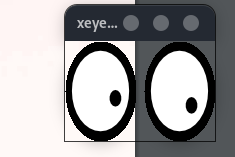
\includegraphics[width=4cm]{images/screen-ssh-td6-2.png}
  \vspace{0.3cm}

  On arrive bien à lancer des applis en mode graphique depuis la machine cli
\end{itemize}
\vspace{0.3cm}

  \subsection{TD-7 : Rebonds}
  \vspace{0.3cm}

\begin{itemize}
  \item \textbf{Configurer .ssh/config avec ProxyJump de manière à pouvoir rebondir automatiquement sur cli lorsque
  vous vous connectez à srv}
  \vspace{0.3cm}

  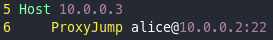
\includegraphics[width=6cm]{images/screen-ssh-td7-1.png}
  \vspace{0.3cm}

  Avec ceci, alice va pouvoir se connecter sur le srv en passant d'abord par la machine cli
\end{itemize}
\vspace{0.3cm}

\begin{itemize}
  \item \textbf{Vous pouvez utiliser la commande who pour vérifier de quelle adresse vous vous connectez.}
  \vspace{0.3cm}

  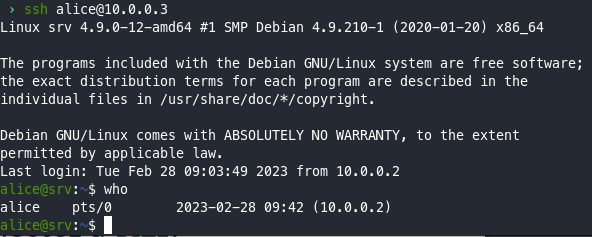
\includegraphics[width=8cm]{images/screen-ssh-td7-2.png}
  \vspace{0.3cm}

  Tout fonctionne, alice passe bien par la machine cli pour se connecter à la machine srv
\end{itemize}
\vspace{0.3cm}

\begin{itemize}
  \item \textbf{Idem en utilisant ProxyCommand au lieu de ProxyJump}
  \vspace{0.3cm}

  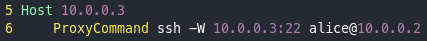
\includegraphics[width=7cm]{images/screen-ssh-td7-3.png}
  \vspace{0.3cm}

  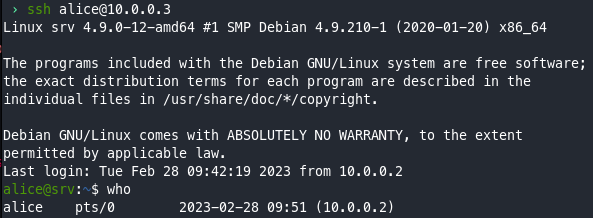
\includegraphics[width=8cm]{images/screen-ssh-td7-4.png}
  \vspace{0.3cm}

  Tout fonctionne, il faut savoir que ProxyCommand est plus sécurisé, car il utilise 2 pairs de clé comparé à ProxyJump
  qui en utilise qu'une seul
\end{itemize}
\vspace{0.3cm}

  \section{Git}

  \subsection{TD-1 : Kickstart}
  \vspace{0.3cm}

\begin{itemize}
  \item \textbf{Créer un nouveau répertoire et y initialiser un repository}
  \vspace{0.3cm}

  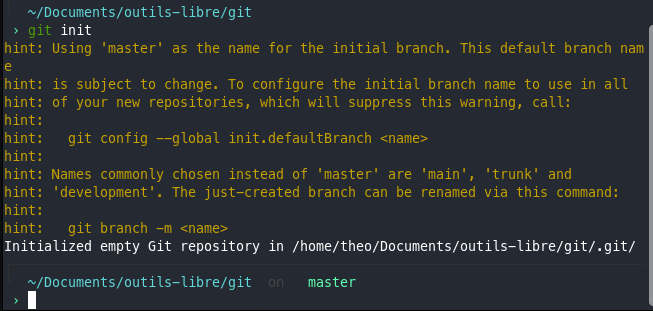
\includegraphics[width=10cm]{images/screen-git-td1-1.png}
\end{itemize}
\vspace{0.3cm}

\begin{itemize}
  \item \textbf{Y copier la configuration Vagrant des TD ssh (Vagrantfile + dossier srv)}
  \vspace{0.3cm}

  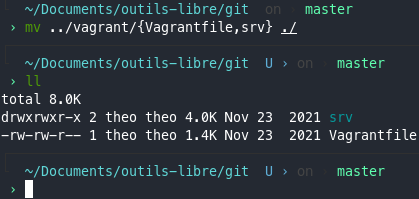
\includegraphics[width=7cm]{images/screen-git-td1-2.png}
\end{itemize}
\vspace{0.3cm}

\begin{itemize}
  \item \textbf{Regarder les modifications détectées par git}
  \vspace{0.3cm}

  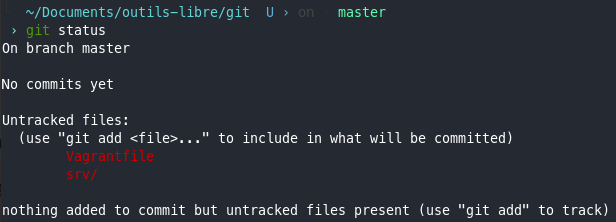
\includegraphics[width=10cm]{images/screen-git-td1-3.png}
  \vspace{0.3cm}

  Git à détécté l'ajout du Vagrantfile et du dossier srv, et il précise qu'ils sont pas add dans la staging area
\end{itemize}
\vspace{0.3cm}

\begin{itemize}
  \item \textbf{Démarrer puis arrêter la configuration Vagrant puis regarder à nouveau les modifications détectées par git,
  que remarque-t-on ? Comment peut-on régler le problème ?}
  \vspace{0.3cm}

  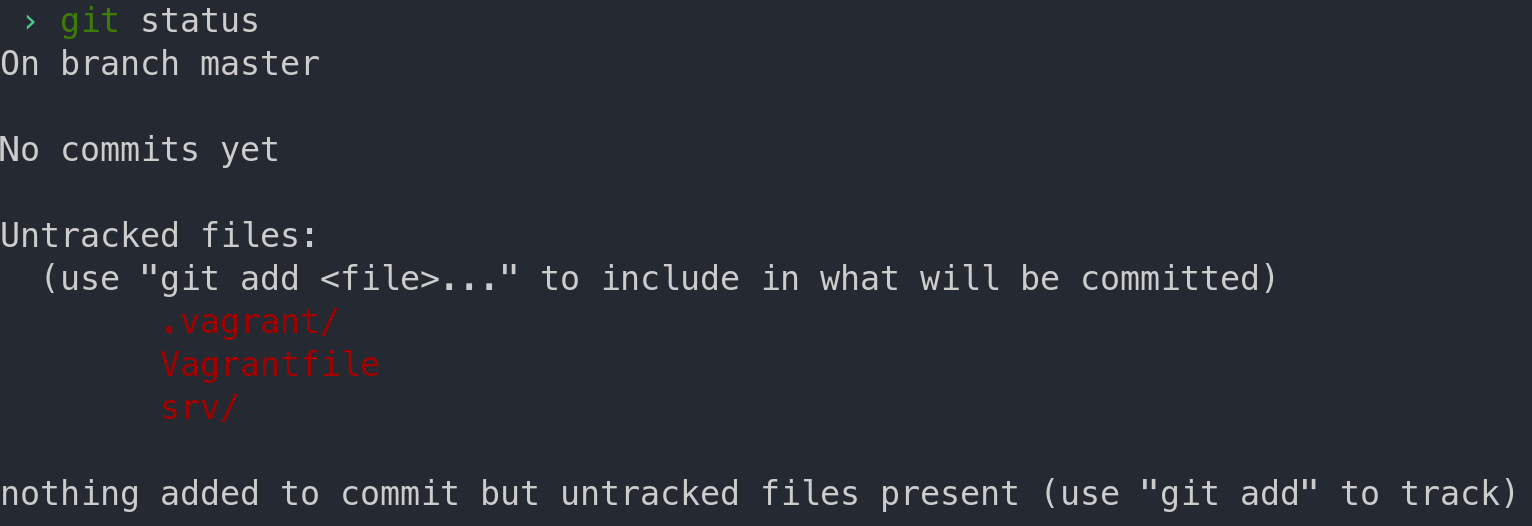
\includegraphics[width=10cm]{images/screen-git-td1-4.png}
  \vspace{0.3cm}

  Git à ajouté le dossier .vagrant/ dans la liste des fichier ajouté récemment, pour éviter cela, on peut écrire un fichier
  .gitignore où on va référencer tous les fichiers qu'on ne veut pas add dans la stagging area :
  \vspace{0.3cm}

  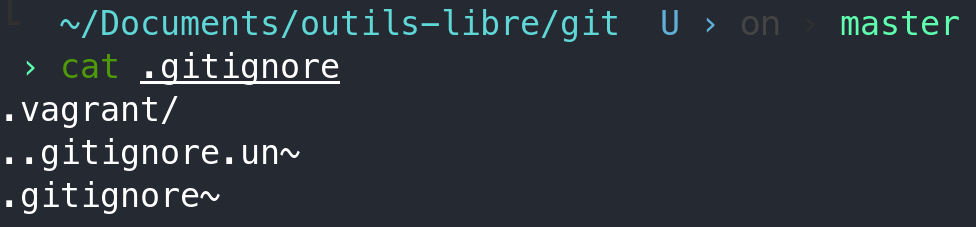
\includegraphics[width=10cm]{images/screen-git-td1-5.png}
  \vspace{0.3cm}

  J'ai ajouté d'autre fichier parasite qui apparaissent à cause de vim
\end{itemize}
\vspace{0.3cm}

\begin{itemize}
  \item \textbf{Ajouter les fichiers Vagrant et commit les modifications, Vérifier que le commit est bien présent et correct}
  \vspace{0.3cm}

  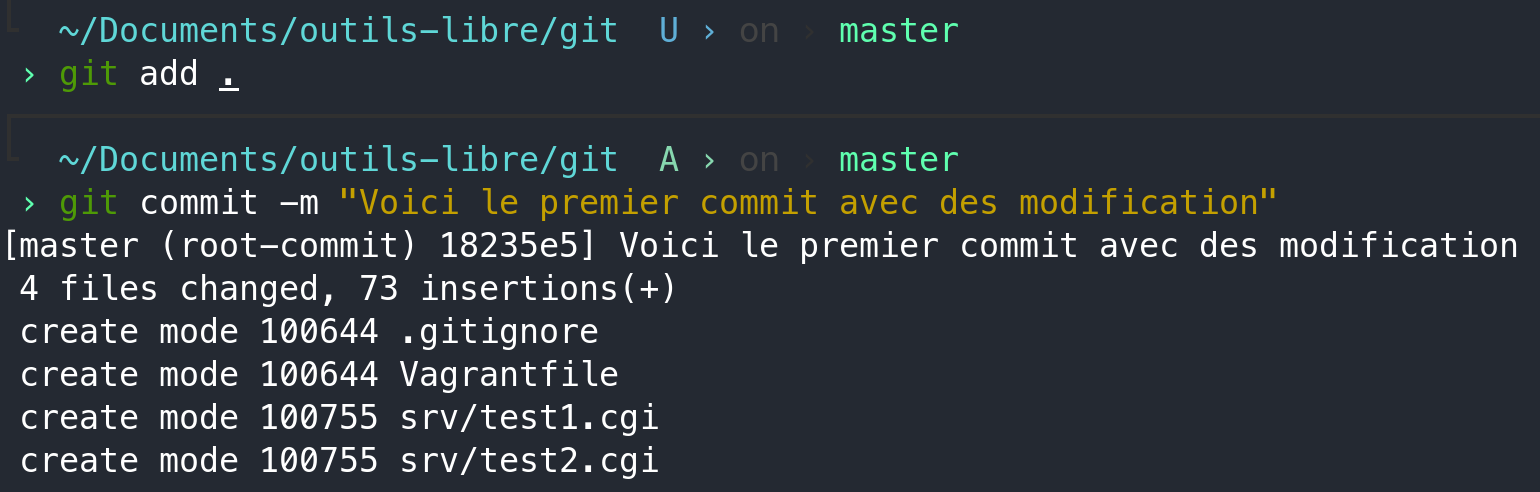
\includegraphics[width=10cm]{images/screen-git-td1-6.png}
  \vspace{0.3cm}

  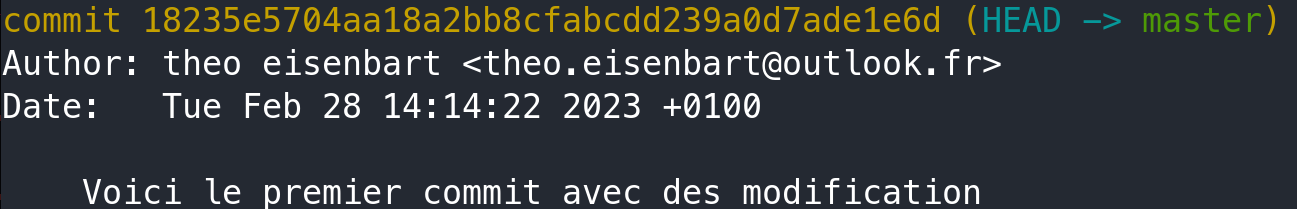
\includegraphics[width=10cm]{images/screen-git-td1-7.png}
  \vspace{0.3cm}

  Tout à bien été commit, j'ai pu en être sur grâce à la commande : \$ git log \newline
  qui permet de voir tous les commit qui on été fait.
\end{itemize}
\vspace{0.3cm}

  \subsection{TD-2 : Les branches}
  \vspace{0.3cm}

\begin{itemize}
  \item \textbf{Créer une nouvelle branche}
  \vspace{0.3cm}

  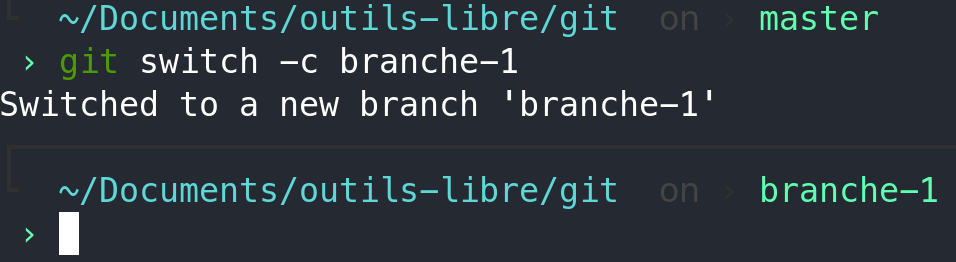
\includegraphics[width=10cm]{images/screen-git-td2-1.png}
\end{itemize}
\vspace{0.3cm}

\begin{itemize}
  \item \textbf{Dans le Vagrantfile, ajouter l'utilisateur patrick}
  \vspace{0.3cm}

  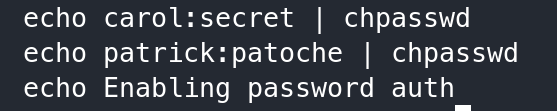
\includegraphics[width=10cm]{images/screen-git-td2-2.png}
\end{itemize}
\vspace{0.3cm}

\begin{itemize}
  \item \textbf{Dans le Vagrantfile, installer php et l'activer sur apache}
  \vspace{0.3cm}

  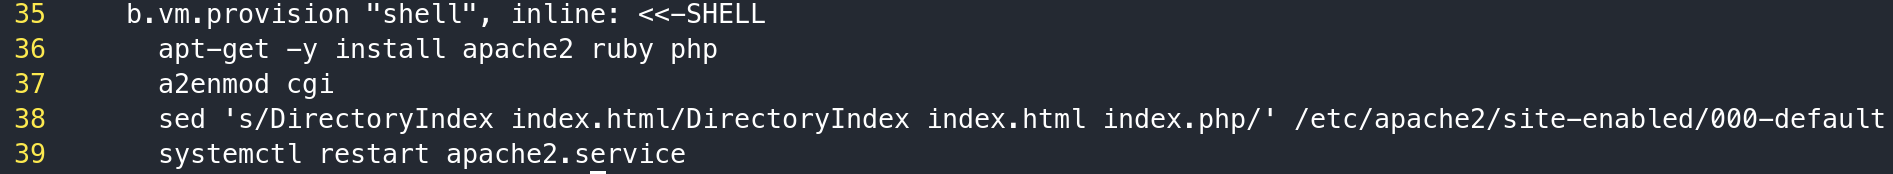
\includegraphics[width=10cm]{images/screen-git-td2-3.png}
\end{itemize}
\vspace{0.3cm}

\begin{itemize}
  \item \textbf{Effectuer 2 commits distincts à l'aide de la commande git add -p}
  \vspace{0.3cm}

  Le premier commit avec l'ajout de l'user patrick :
  \vspace{0.3cm}

  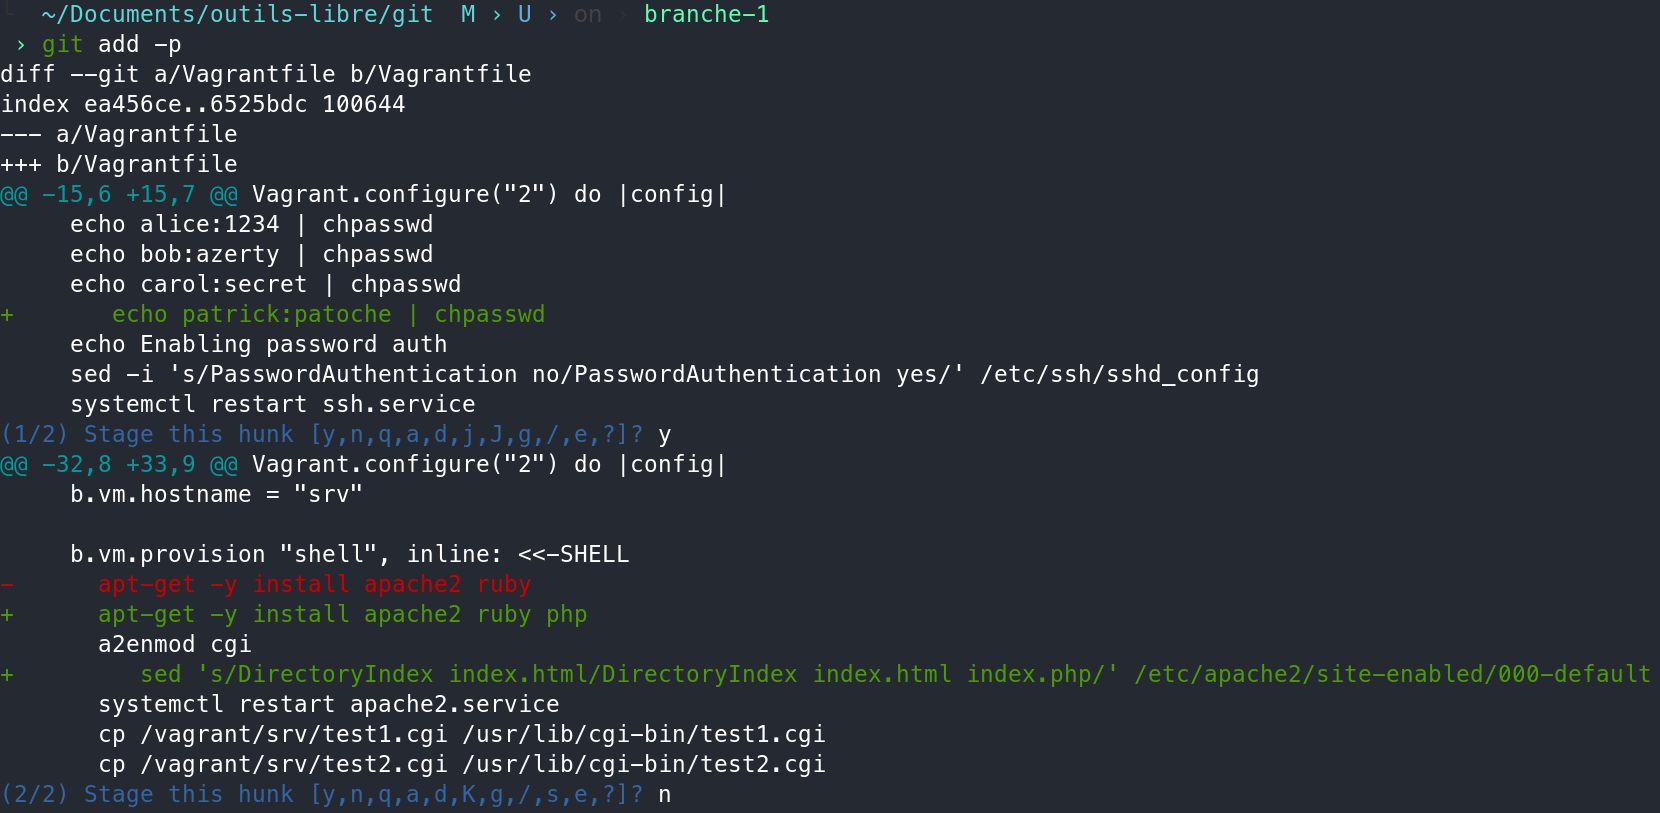
\includegraphics[width=13cm]{images/screen-git-td2-4.png}
  \vspace{0.3cm}

  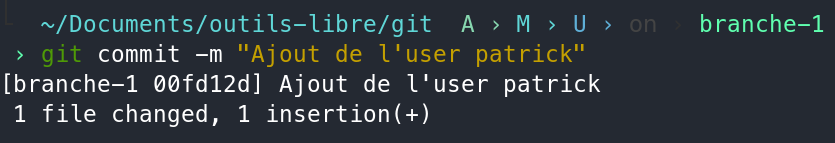
\includegraphics[width=10cm]{images/screen-git-td2-5.png}
  \vspace{0.3cm}

  Et le deuxième commit avec l'ajout de php :
  \vspace{0.3cm}

  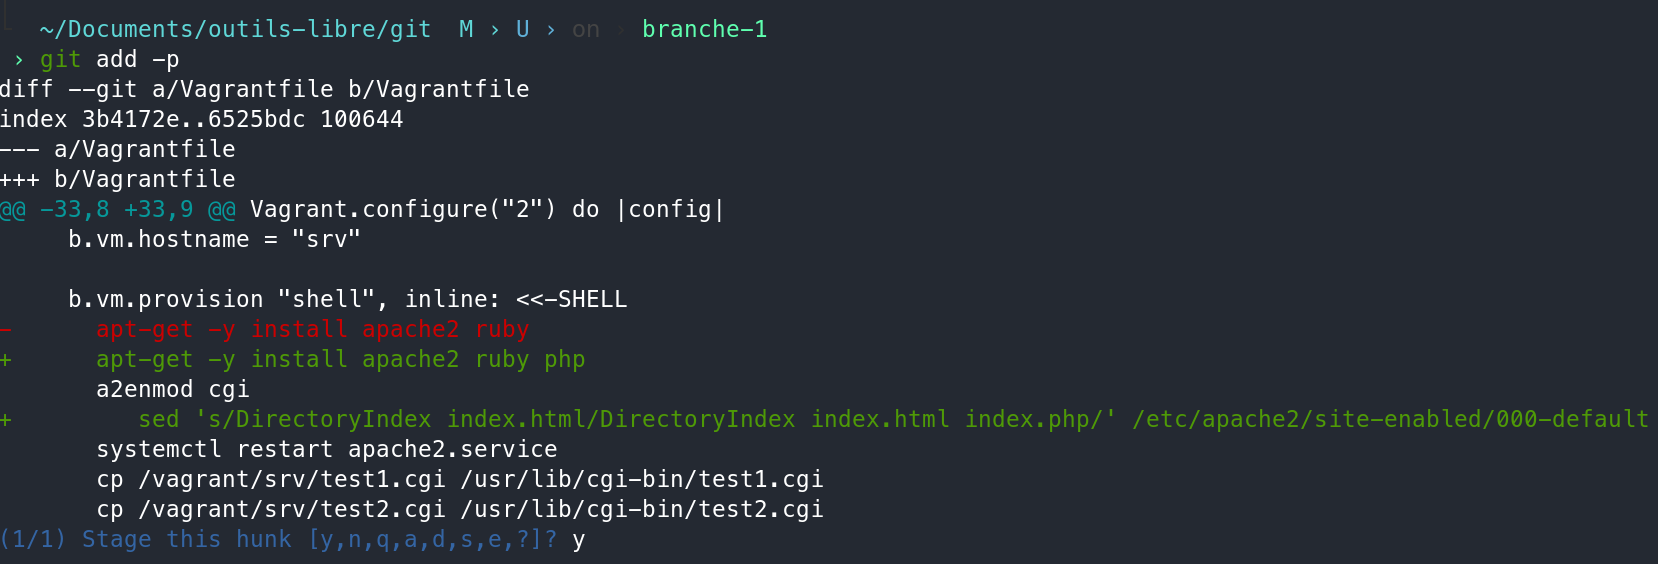
\includegraphics[width=13cm]{images/screen-git-td2-6.png}
  \vspace{0.3cm}

  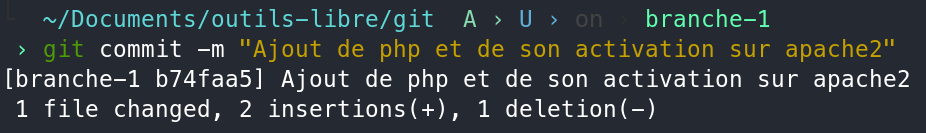
\includegraphics[width=10cm]{images/screen-git-td2-7.png}
  \vspace{0.3cm}

  On peut s'assurer que les commits on bien été fait en utilisant la commande : \newline
  \$ git log
  \vspace{0.3cm}

  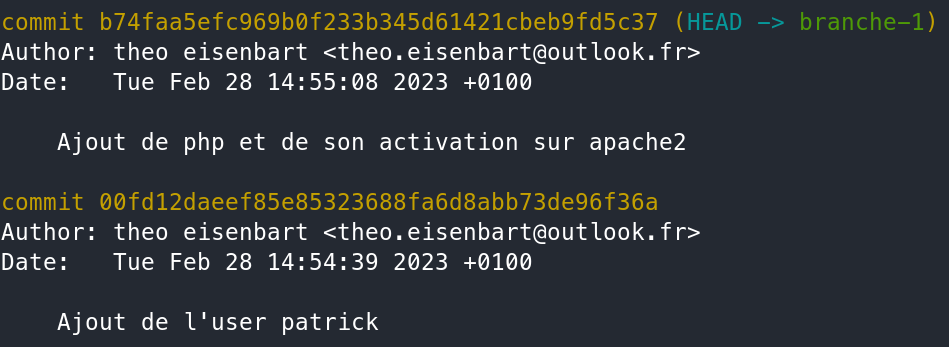
\includegraphics[width=10cm]{images/screen-git-td2-8.png}
\end{itemize}

\begin{itemize}
  \item \textbf{Revenir à la branche main , quel est l'état de votre working directory ?}
  \vspace{0.3cm}

  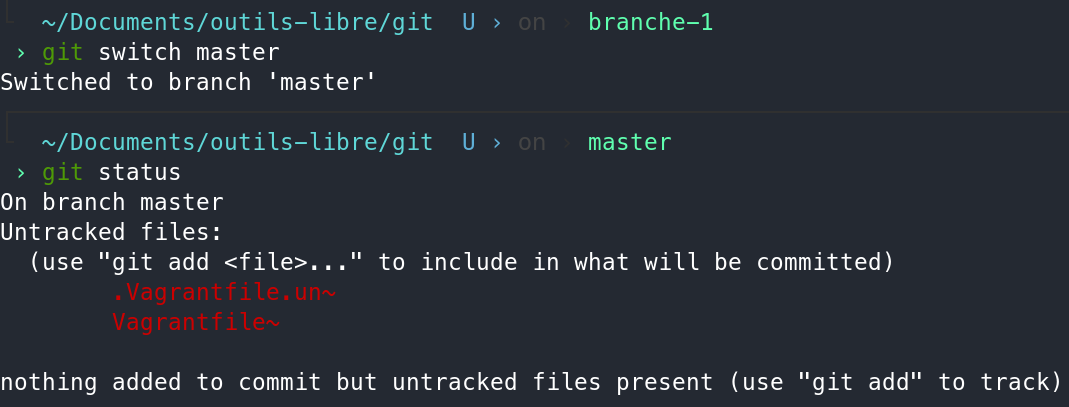
\includegraphics[width=10cm]{images/screen-git-td2-9.png}
  \vspace{0.3cm}

  A part les fichier de merde dû à vim, rien n'a changer
\end{itemize}
\vspace{0.3cm}

\begin{itemize}
  \item \textbf{Intégrer les modification de code de l'exercice précédent dans main}
  \vspace{0.3cm}

  \includegraphics[width=10cm]{images/screen-git-td2-10.png}
\end{itemize}
\vspace{0.3cm}

\begin{itemize}
  \item \textbf{Inspecter le commit de merge, y'a t'il des specificités ?}
  \vspace{0.3cm}

  \includegraphics[width=10cm]{images/screen-git-td2-11.png}
  \vspace{0.3cm}

  Oui, il est noté que ces commits proviennent de la branche "branche-1"
\end{itemize}
\vspace{0.3cm}

\begin{itemize}
  \item \textbf{Est-ce que la branche que vous avez créé existe toujours ? Qu'est-ce qu'on en fait ?}
  \vspace{0.3cm}

  Grâce à la commande : \newline
  \$ git branch \newline
  on peut voir toute les branches de notre repo local :
  \vspace{0.3cm}

  \includegraphics[width=2cm]{images/screen-git-td2-12.png}
  \vspace{0.3cm}

  Donc la branche "branche-1" éxiste encore, on peut la supprimer, mais le mieux serait de la garder pour avoir un
  historique des commits
\end{itemize}
\vspace{0.3cm}

  \subsection{TD-3 : Les conflits}
  \vspace{0.3cm}

\begin{itemize}
  \item \textbf{Créer une nouvelle branche forward-new-port à partir de main}
  \vspace{0.3cm}

  \includegraphics[width=8cm]{images/screen-git-td3-1.png}
\end{itemize}
\vspace{0.3cm}

\begin{itemize}
  \item \textbf{Sur forward-new-port : modifier le Vagrantfile pour forward le port 80 vers 8081 pour srv, puis commit}
  \vspace{0.3cm}

  \includegraphics[width=8cm]{images/screen-git-td3-2.png}
\end{itemize}
\vspace{0.3cm}

\begin{itemize}
  \item \textbf{Sur main : modifier le Vagrantfile pour forward le port 80 vers 8080 pour srv, puis commit}
  \vspace{0.3cm}

  \includegraphics[width=8cm]{images/screen-git-td3-3.png}
\end{itemize}


\end{document}
